\documentclass[12pt, a4paper, twoside, table, xcdraw]{report}

%% Language and font encodings
\usepackage[utf8]{inputenc}

\usepackage[english]{babel}
\usepackage[T1]{fontenc}

% \setmainlanguage{english}
% \usepackage{svg}

\usepackage{listings}
\usepackage{textcomp}
\usepackage{longtable} \usepackage{multirow}
\usepackage[page,toc,titletoc,title]{appendix}
\usepackage{tocloft}
\usepackage{blindtext} % \usepackage{titlesec}
% \titleformat{\chapter}{}{}{0em}{\bf\LARGE}


\usepackage[spaces,hyphens]{url}


\usepackage[normalem]{ulem}
\useunder{\uline}{\ul}{}


\usepackage{graphicx}
% \usepackage[table,xcdraw]{xcolor}
% If you use beamer only pass "xcolor=table" option, i.e. \documentclass[xcolor=table]{beamer}
\usepackage{lscape}

%% Sets page size and margins
\usepackage[a4paper,top=3cm,bottom=2cm,left=3cm,right=3cm,marginparwidth=1.75cm]{geometry}

% Set subsubsubsection
\setcounter{tocdepth}{4} 
\setcounter{secnumdepth}{4}

\usepackage[table,xcdraw]{xcolor}

% Set style
\usepackage{listings}
\usepackage{xcolor}

\definecolor{codegreen}{rgb}{0,0.6,0}
\definecolor{codegray}{rgb}{0.5,0.5,0.5}
\definecolor{codepurple}{rgb}{0.58,0,0.82}
\definecolor{backcolour}{rgb}{0.95,0.95,0.92}



%% Useful packages
\usepackage{svg}
\usepackage{amsmath}
\usepackage{setspace}
% \usepackage[colorinlistoftodos]{todonotes}
\usepackage[colorlinks=true, allcolors=blue]{hyperref}
\graphicspath{{./images/}}

\title{Title}

\onehalfspacing

\begin{document}
\begin{titlepage}

\newcommand{\HRule}{\rule{\linewidth}{0.5mm}} % Defines a new command for the horizontal lines, change thickness here

%----------------------------------------------------------------------------------------
%	LOGO SECTION
%----------------------------------------------------------------------------------------
\begin{figure}
    \centering
    
\includegraphics[width=5.5cm]{./title/Logo20.png}
    \hspace{1cm}
    
\includegraphics[width=5.5cm]{./title/fra_uas_logo.png}
\end{figure}


% Include a department/university logo - this will require the graphicx package

 
%----------------------------------------------------------------------------------------

\center % Center everything on the page

%----------------------------------------------------------------------------------------
%	HEADING SECTIONS
%----------------------------------------------------------------------------------------

\textsc{\LARGE INTERNSHIP REPORT}\\[1.5cm] 
\textsc{\Large Internship period:}\\[0.5cm] 
\textsc{\large 01/03/2023 - 10/06/2023}\\[0.5cm] 

%----------------------------------------------------------------------------------------
%	TITLE SECTION
%----------------------------------------------------------------------------------------
\makeatletter
\HRule \\[0.6cm]
{ \huge \bfseries Latency and Fault Tolerance: An Analysis of Mutual Exclusion Algorithms in Distributed Systems}\\[0.2cm] % Title of your document
\HRule \\[1.5cm]
 
%----------------------------------------------------------------------------------------
%	AUTHOR SECTION
%----------------------------------------------------------------------------------------

\begin{minipage}{0.4\textwidth}
\begin{flushleft} \large
\emph{Author:}\\
Huynh Minh Triet - 17447\\

\end{flushleft}
\end{minipage}
~
\begin{minipage}{0.55\textwidth}
\begin{flushright} \large
\emph{Instructors:} \\
M.Sc. Lukas Atkinson\\
Prof. Dr. Martin Kappes 
\end{flushright}
\end{minipage}\\[2cm]
\makeatother

%----------------------------------------------------------------------------------------
%	DATE SECTION
%----------------------------------------------------------------------------------------

{\large \today}\\[2cm] % Date, change the \today to a set date if you want to be precise

\vfill % Fill the rest of the page with whitespace

\end{titlepage}

\cleardoublepage

\tableofcontents

% Put all of your chapters here
% \chapter{\centering Introduction}

\section{Motivation}
More and more the current trend of software development is that of a departure 
from monolithic architecture to that of microservices this is done for scalability 
and flexibility. Yet despite all the benefits that microservices that brings
this shift in paradigm also brings with it a host of distributed system complexities.

However, there is still a lack of tooling to help with quality assurance

\section{State of The Art}

\section{Overview}


% \chapter{\centering Presentation of the company}


\includegraphics[width=\textwidth]{research_group_logo.png} \\

The Network Security, Information Security, and Data Protection Research Group 
operates under the astute leadership of Prof. Dr. Kappes. The group's principal 
focus is on the research and development of advanced network security solutions 
for future generations. In addition to theoretical research, the group also offers
practical solutions to third parties, including private companies and governmental agencies.

During this research period, I have the privilege of working under the supervision 
of Lukas Atkinson (M.Sc.), with additional support from Prof. Dr. Kappes. Our 
collaboration is entirely virtual, involving 2-3 meetings per week to discuss 
current progress and to exchange ideas and guidance

\chapter{\centering Internship position}


\includegraphics[width=\textwidth]{research_group_logo.png} \\

I completed my internship at The Research Group for Network Security at\\
Frankfurt University of Applied Sciences.\\ 

Overall, my work during the internship period can be divided into roughly three phases:
\begin{itemize}
  \item Prototyping Phase: A prototype of a distributed system communicating via HTTP 
    is built.
  \item Fault Injection and Fuzzy Testing Phase: A method of fault injection and fuzzy testing is developed
    to test the aforementioned system.
  \item Data Collection and Statistical Analysis: Data resulted from the testing of the system is gathered
    and compiled to create statistical analysis of the system.
\end{itemize}


During this research period, I have the privilege of working under the supervision 
of Lukas Atkinson (M.Sc.), with additional support from Prof. Dr. Kappes. Our 
collaboration is entirely virtual, involving 2-3 meetings per week to discuss 
current progress and to exchange ideas and guidance.





% \chapter{\centering Applied Technologies}

Overall the technologies used in the internship's project can be divided into
three categorizes: Prototyping, Testing, and Data visualization

\section{Prototyping}

\subsection{Distributed System}


\subsection{Python}
Python is a high level interpreted language, it is dynamically-typed, and garbage-collected.
The reason for python being chosen because it eases of development stemming from 
python easy to read syntax and conciseness. Also, because there are state-of-the-art
testing frameworks such as hypothesis and other data visualization such as Matplotlib
that is widely used and documented make python the most well suited option for 
this project.

% \subsection{JSON}

\subsection{HTTP}
Since the scope of the internship investigation is about HTTP communication and to mimic 
most closely to real life production scenario HTTP is chosen as the main communication 
protocol between the nodes in the system, more specifically we will be using HTTP/2 with 
TCP as the transport layer.

HTTP functions in a request response manner to the in the client-server model, 
in which a client will make a request to the server and awaits for a response 
from the server, all participants can include in their request or response 
an optional payload which in this project is encoded in the JSON format.

\subsection{Flask}

\section{Testing}

\subsection{pytest}

\subsection{hypothesis}

\chapter{\centering Background}

Originally software architecture were monoliths where a single component is 
responsible for all the application's logic. However, over time especially how 
the issue of horizontally scaling the infrastructure become more and more pressing 
as the demand of the modern world for modern technology is also increasing for now
the solution to solve them is microservices.

This means that software systems are increasingly becoming distributed, but this 
also brings with it increasing challenges in ensuring the reliability and 
security of the system.

By introducing extra components into a software system also increases the amount 
of failure points that are possible. For example latency that are small in 
testing environment could become very substantial in the production environment 
consisting of hundreds of nodes.

This internship work aim is to show how much latency and error affects a distributed
system by doing fault injection, a technique where developers deliberately introduce
error into the system to see whether the system's response is sufficiently resilient 
or robust.

Furthermore, in the during the building of the prototype a library called Hypothesis
will be used for fuzzy based testing ensuring the correctness of the system. 

In addition, fuzzy based testing is also used to randomly inject faults into the system
to mimic the arbitrary nature of real world faults occurrences and avoiding covering
only the typically expected faults or "happy paths" \cite{happy_path}.

% \chapter{\centering Project's architecture}
\label{chap:project_arch}


\chapter{\centering Implementation}
\section{Prototyping Phase}

For the three months internship about the first one and a half months was spent 
on learning and developing the distributed system.

\subsection{Architecture of the prototype}

The prototype was built using the Python programming language along 
with Flask \cite{flask} a popular microframework built on top of Werkzeug WSGI 
toolkit, the Jinja template engine, and the Click CLI toolkit. It is classified
as a microframework because it does not provide much of the features commonly used
in web application development by default. 

However, this is perfect for the internship project as the goal was to only build
a working prototype of communicating nodes without any graphical user interface.

As shown in the figure \ref{fig:prototype_architecture} shows an overview of the prototype 
consisting a minimum of 4 clients nodes, 1 proxy, 1 database or resource manager, and 1 logger.

\begin{figure}[htbp]
  \centering
  \includesvg{images/prototype_architecture.svg} 
  \caption{Overview of prototype Architecture}
  \label{fig:prototype_architecture}
\end{figure}

The figure in \ref{fig:prototype_architecture} is the final version of the prototype.
During this phase of the internship the prototype was developed in an incremental
manner with first the clients and resource being added, then comes the proxy and 
finally the logger.

Every client has a RESTful API layer that allows for communication and data transfer 
between each other using HTTP and JSON as the encoding format for data.

\subsubsection{Client}

Since the entire prototype is run on a single local host each client is actually 
a single process running concurrently to each others. 

Each client has a HTTP endpoint which response to a specific HTTP verb such as
GET, PUT, or POST this is called a view in Flask:

\begin{listing}[!ht]
  \begin{minted}{python}
  @bp.route("/<string:resource_id>/request", methods=["POST"])
  async def request_resource(resource_id: str) -> tuple[str, int]:
      data = request.get_json()
      delay_time: str = data["delay_time"]
      # ...
  \end{minted}
\caption{function signature of a client}
\label{code:signature}
\end{listing}

In addition, as we can see from the code snippet \ref{code:signature}  each view is having the word 
async in the front to indicate that this is an asynchronous function. 

The reason for the async keywords is to allow for the use of the keyword 
\textit{await} to handle the scenario where there are multiple messages to be 
sent. If that was done without concurrency then the entire process is hung 
and have to wait until the HTTP request is sent and responded to which takes a 
lot of time.

\begin{listing}[!ht]
\begin{minted}{python}
coroutines = []

for target_url in CLIENT_URL:
    coroutine = session.post(
        # ...
        proxy=PROXY_URL,
    )
    coroutines.append(coroutine)

await asyncio.gather(*coroutines)
\end{minted}
\caption{Multiple requests being sent simultaneously}
\label{code:multiple_requests}
\end{listing}


The code in \ref{code:multiple_requests} is putting all the coroutines of sending the HTTP request into 
an array. By using \textit{asyncio.gather()} it will await for all and finished
when all coroutines are finished.


\subsubsection{Proxy}

The existence of the proxy is to inject fault into the system and monitor to 
generate the necessary data for analysis.

Inside the snippet of \ref{code:multiple_requests} there is the line 
\textit{proxy=PROXY\_URL}
similarly for all HTTP request and response in the prototype they all have this line 
as a part of the option when sending HTTP requests, this is done to route all 
communication via the proxy.

This is done so that the process of fault injection, for more information on fault injection and what it is
please refer to \ref{subsec:fault_injection}.

Initially when the proxy is built it was run using the Flask default development 
server \cite{flask_dev_server}. 

However, there is a problem with this approach in our goal to obtain the correct 
data points, the proxy soon proves to be one of the big bottleneck.

This is because the clients are communicating using aiohttp which sends all the 
message asynchronously, which means more or less the request are being sent 
simultaneously.

However, the original proxy was running on Flask's development server which is 
only single threaded. This resulted in, although the request is being sent sequentially
one after another due to the proxy incapable of handling concurrent requests.

to solve this issue we switched over from the development server to gunicorn,
which allows for use to use multiple workers at the same time for the proxy.

\begin{listing}[!ht]
  \begin{minted}{bash}
gunicorn --reload -w 4 -b 127.0.0.1:5001 "proxy:create_app()"
  \end{minted}
  \caption{Running gunicorn with 4 workers}
\end{listing}

Since the proxy is now severed by at least 4 workers, one for each client, each
client's HTTP request are now being sent concurrently as initially intended.

\subsubsection{Logger}

To gather the information needed, there is a process constantly running called 
the logger. The logger has two endpoints:

First is the log endpoint: 

\begin{listing}[!ht]
  \begin{minted}{python}
  @app.route("/<string:resource_id>/log", methods=["PUT"])
  def log(resource_id: str):
  \end{minted}
  \caption{Code snippet of the logger's log endpoint}
  \label{code:logger_log}
\end{listing}

The endpoint \ref{code:logger_log} is being accessed at the start of the client request, meaning 
when the client node shows an initial interest in accessing the resource and is called again when the
resource is actually been acquired by that client. 

Each client carries along with its request a Unix timestamp that at the time of calling 
that request. 


When the logger is first called it will log the start time of that request:

\begin{listing}[!ht]
  \begin{minted}{python}
   latency_dict: dict[str, float] = {}
  \end{minted}
  \caption{in memory dictionary to store the latency}
  \label{code:latency_dict}
\end{listing}


When the log endpoint is being called a second time, the logger will take the time 
that the second request is being called subtract the time stored in the \textit{latency\_dict}
to obtain the latency.

\begin{listing}[!ht]
  \begin{minted}{python}
  latency_tally: list[dict[str, float]] = []
  \end{minted}
  \caption{The resulted latency is stored in a list}
  \label{code:latency_tally}
\end{listing}

\textit{latency\_tally} is a list of dictionaries, each dictionary keys are the 
name of that client, e.g., client\_1 and the value 0.02 is the latency of that client.


\subsubsection{Resource Manager}
\label{subsubsec:resource_manager}

Resource manager is another process where the client contact to either lock or
delete a particular resource.

\begin{listing}[!ht]
  \begin{minted}{python}
@bp.route("/<string:resource_id>/lock", methods=["PUT"])
def lock(resource_id: str):
  # ...

@bp.route("/<string:resource_id>/lock", methods=["DELETE"])
def unlock(resource_id: str):
  # ...
  \end{minted}
\end{listing}

In addition, there is also another endpoint to check whether a race condition 
has occurred:

\begin{listing}[!ht]
  \begin{minted}{python}
@bp.route("/<string:resource_id>/is_lock", methods=["GET"])
def check_locking_status(resource_id: str):
  # ...
  \end{minted}
\end{listing}

All the resources are stored in memory using a class 

\begin{listing}[!ht]
  \begin{minted}{python}
@dataclass(slots=True)
class ServerState:
    race_condition: bool = False
    resource: dict[str, bool] = field(default_factory=dict[str, bool])
  \end{minted}
\end{listing}



\section{Fault Injection and Property Based Testing Phase}


\subsection{Property Based Testing}
Once all the algorithms are finished implementing each of the algorithms in 
\ref{chap:algorithms} we need to ensure the correctness of each algorithm, and to
do this we used a property based testing framework called \textit{Hypothesis}.

But before we go into Hypothesis a quick introduction into the history of fuzzy testing.
Fuzzy testing was first introduced in \cite{OG_fuzzy_testing}, where researcher
gave Unix utilities such as awk, grep, etc. a lot of random inputs to see if they crash or 
result in undefined behavior.

Overtime, fuzzy testing developed and mature to give us a more advance method called
property based testing such as \textit{Quickcheck} \cite{quickcheck}, in which the strategy is still 
to generate random input and feed it into the program under testing but this 
time certain property are being tested to see if they hold across the runtime 
and not just a crash. Furthermore, once a property also called invariant has 
been violated they can be shrunk to a minimal failing example, the smallest test 
case that will also result in the same behavior. 

The property based testing that in used in this project is \textit{Hypothesis} an
implementation of \textit{Quickcheck} in Python but also come with some other features
such as caching past mistakes and stateful testing.

\subsubsection{Basic Hypothesis Tests}
\label{subsubsec:basic_hypothesis_tests}


\begin{listing}[!ht]
  \begin{minted}{python}
from hypothesis import given, strategies as st
@given(
    resource_id=st.sampled_from(["A", "B"]),
    client_port=st.integers(min_value=5002, max_value=5003),
)
  # ...
  \end{minted}
  \caption{Hypothesis python decorator}
  \label{code:hypothesis_decorator}
\end{listing}

The decorator above in listing \ref{code:hypothesis_decorator} set up the randomization of the input, the testing case above 
means choose a random client in each of the four client to lock on either resource 
type "A" or "B".

\begin{listing}[!ht]
  \begin{minted}{python}
#...
def test_one_client_lock_and_delete(
    setup_ricart_agrawala,
    resource_id: str,
    client_port: int,
):
  #...
  \end{minted}
  \caption{Test case function signature}
  \label{code:test_case_signature}
\end{listing}

The test signature's in listing \ref{code:test_case_signature} parameter \textit{resource} 
and \textit{client\_port} is being provided by the Hypothesis decorator 
in listing \ref{code:hypothesis_decorator}. The parameter \textit{setup\_ricart\_agrawala}
is a pytest's fixture which does the setup and tear down of the clients, proxy, logger 
and resource manger at the beginning and end of every test to ensure a blank state 
and a testing environment that is not influenced by previous runs.

\begin{listing}[!ht]
  \begin{minted}{python}
    #...
    response = requests.post(
        f"http://127.0.0.1:{client_port}/{resource_id}/lock",
        timeout=TESTING_TIMEOUT,
    )

    assert response.status_code == 200

    response = requests.delete(
        f"http://127.0.0.1:{client_port}/{resource_id}/lock",
        timeout=TESTING_TIMEOUT,
    )

    assert response.status_code == 200
  \end{minted}
  \caption{Body of the test case}
  \label{code:test_case_body}
\end{listing}


The testing logic in listing \ref{code:test_case_body} is after each client lock or delete
on a particular resource, a check for the request response's status code is equal 
to 200, mean successfully executed by using python's \textit{assert}.

\subsubsection{Stateful Testing}
\label{subsubsec:stateful_testing}
In the section above in listing \ref{subsubsec:basic_hypothesis_tests} \textit{Hypothesis} 
does only randomization of the inputs for each test case. However, during the process
of developing the prototype for this project the majority of the bugs found where
not the result of randomizing the input but from the random ordering of client 
locking or deleting a resource, this is where Stateful testing comes in.


Stateful testing, or model based testing, deploys a state machine with a set of 
predefined \textit{@rule} and the state machine will try to find the sequence
of \textit{@rule} that will result in a failure.

\begin{listing}[!ht]
  \begin{minted}{python}
class MutexLocking(RuleBasedStateMachine):
  #... 
    @initialize()
    def inject_fault(self):
        #...
  def teardown(self):
  #...
      requests.post(
          f"{SERVER_URL}reset",
          timeout=TESTING_TIMEOUT,
      )
 \end{minted}
 \caption{Initialization and teardown of the state machine}
 \label{code:init_teardown_state_machine}
\end{listing}

The code in listing \ref{code:init_teardown_state_machine} does some initialization to set
up and \textit{teardown} to reset the testing environment similar to pytest's fixture 
in \ref{code:test_case_signature}.

\begin{listing}[!ht]
  \begin{minted}{python}
    @rule(
        resource_id=st.sampled_from(["A", "B"]),
        client_port=st.integers(min_value=5002, max_value=5005),
    )
    def test_lock(
        self,
        resource_id: str,
        client_port: int,
    ):
    # ...

    #... 
    def test_unlock(#...)
    #... 
  \end{minted}
  \caption{Rules for locking and unlocking resources}
  \label{code:rule}
\end{listing}

Each of the rules in listing \ref{code:rule} will be run in an arbitrary order by hypothesis.

\begin{listing}[!ht]
  \begin{minted}{python}
    @invariant()
    def test_no_race_condition(self):
        response = requests.get(
            f"{SERVER_URL}race",
            timeout=TESTING_TIMEOUT,
        )
  \end{minted}
  \caption{Invariant checking for race condition on the resource manager}
  \label{code:invariant}
\end{listing}

To ensure a certain property is being held, in the example in listing \ref{code:invariant} is that there is 
no race condition ever happens on the resource manager \ref{subsubsec:resource_manager}.
We specified an invariant called \textit{test\_no\_race\_condition} which will be run 
after each rule, checking whether it has been violated.


\section{Data Collection and Graph Generation}

Every time a latency test completes—this is a test designed to evaluate the impact 
of delay on the prototype's performance—the testing mechanism contacts the logger 
via the /stat endpoint. The test data collected is then written into a JSON file:
  
\begin{listing}[H]
  \begin{minted}{json}
[
  {
    "delay_time": "0.0",
    "latency": 0.04399871826171875
  },
  ...
]
  \end{minted}
  \caption{Latency data obtain from the logger}
  \label{code:latency_json}
\end{listing}

The resulting JSON file follows the naming convention: algorithm\_name\_\%Y-\%m-\%d\_\%H-\%M-\%S.json. As an example, a file could be named as maekawa\_2023-06-07\_09-21-36.json, where 'maekawa' is the name of the algorithm being tested, and the rest of the filename corresponds to the timestamp (date and time) when the file was first created.

Utilizing the value of \textit{delay\_time} as the x-axis and \textit{latency} 
as the y-axis from the data outlined in \ref{code:latency_json}, tools such as 
numpy and matplotlib enable us to create illustrative graphs. These visualizations can provide a clearer understanding of the data:

\begin{figure}[H]
  \centering
  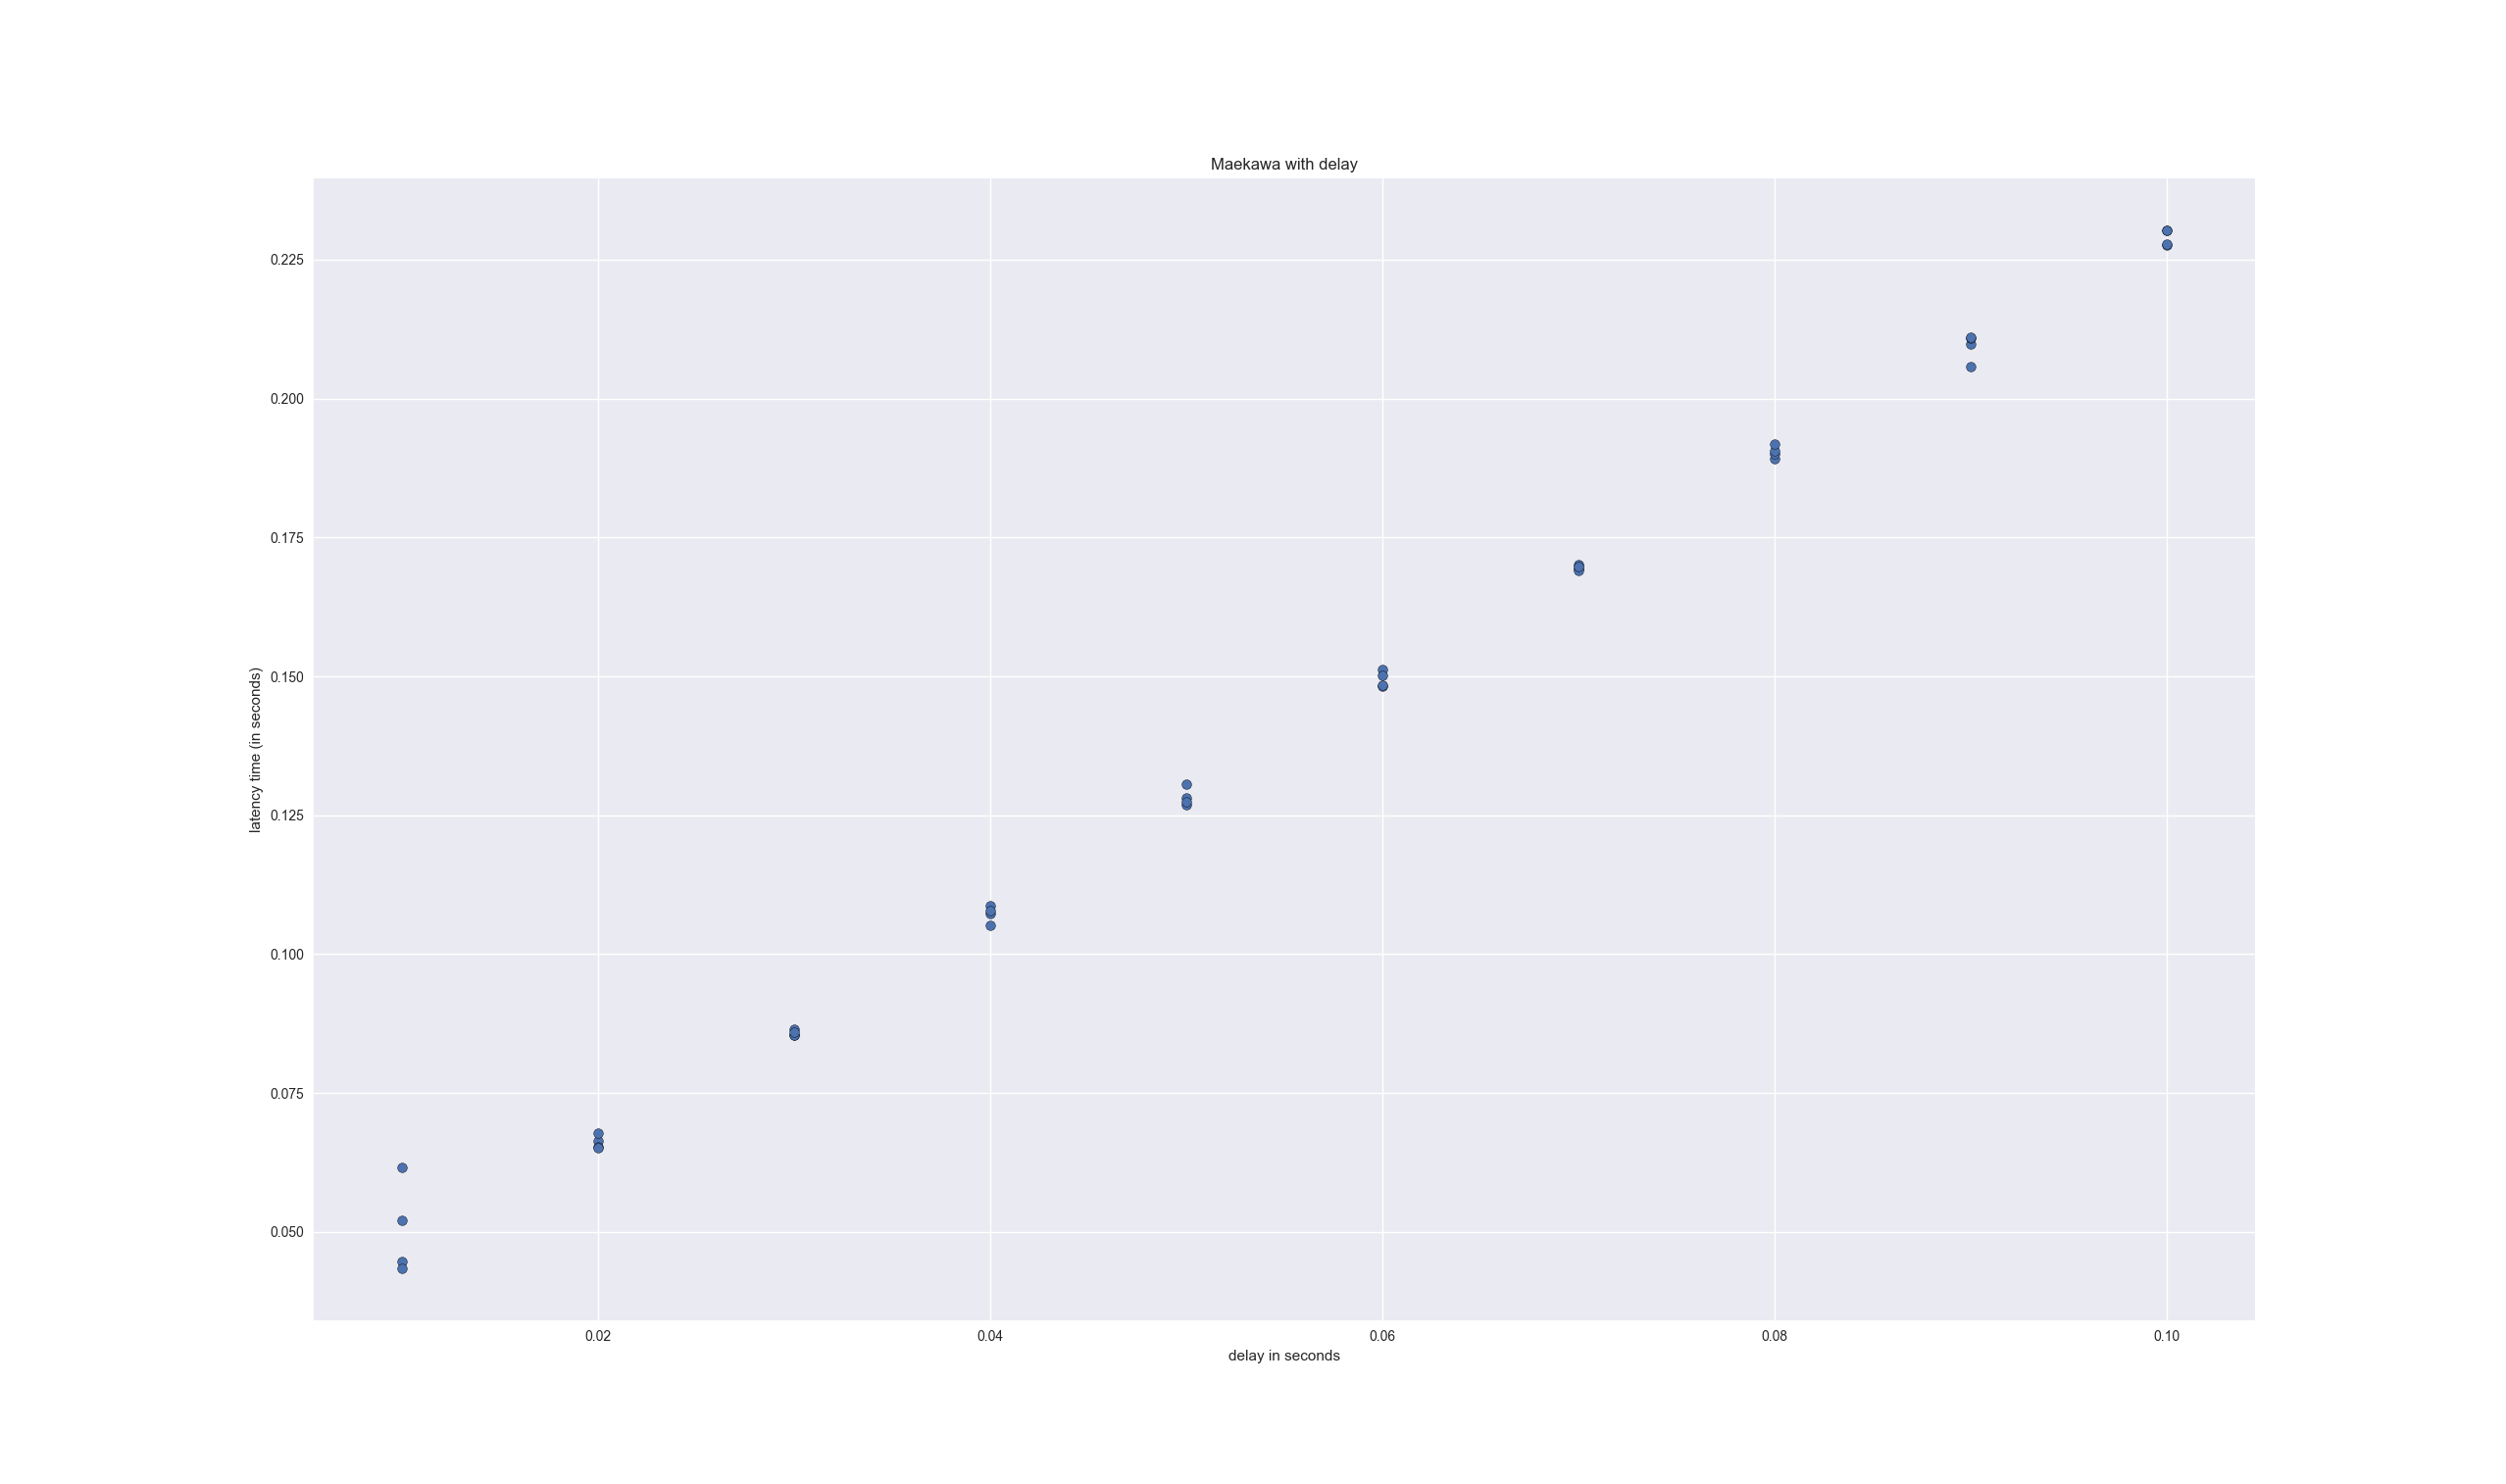
\includegraphics[width=\linewidth,height=\textheight,keepaspectratio]{maekawa_delay.png}
  \caption{Scatter plot between latency and delay in Maekawa algorithm}
\end{figure}

\begin{figure}[H]
  \centering
  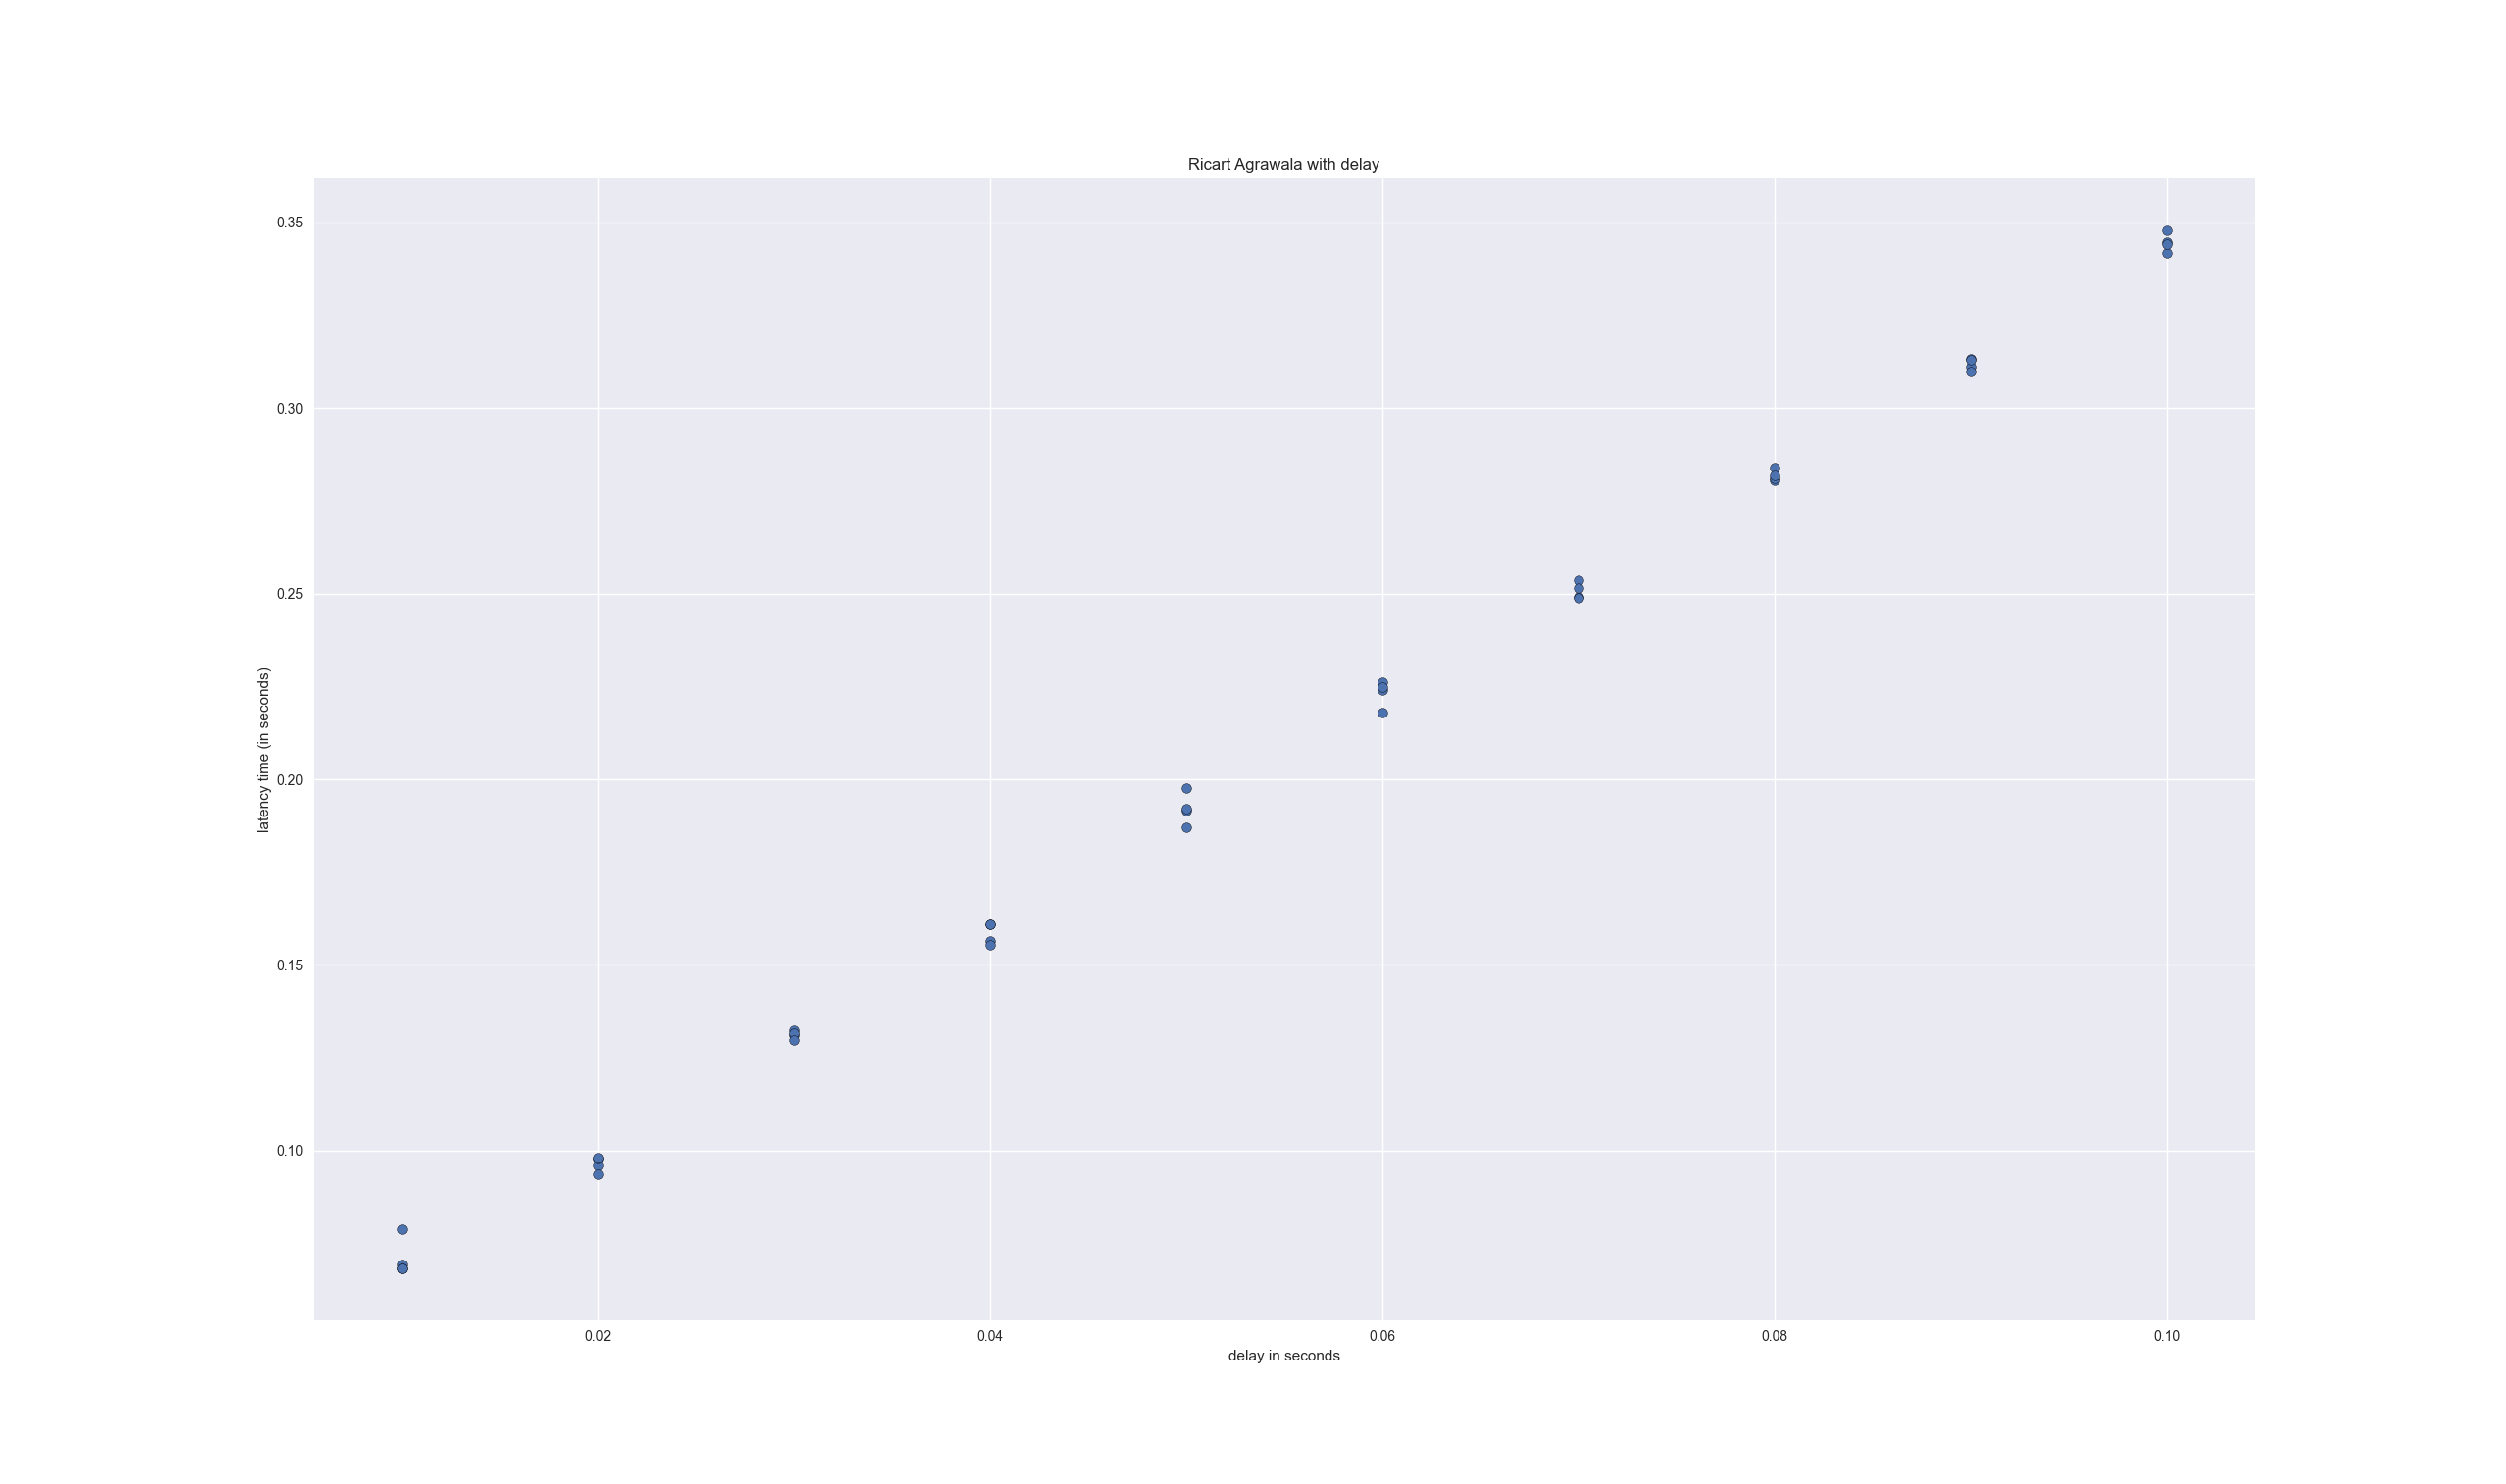
\includegraphics[width=\linewidth,height=\textheight,keepaspectratio]{ricart_agrwala_delay.png}
  \caption{Scatter plot between latency and delay in Ricart-Agrawala algorithm}
\end{figure}

Due to time constraints during the three-month internship phase, we were unable 
to conduct further exploration with error type fault and perform more extensive statistical tests.


\chapter{\centering Distributed Mutex Algorithms}
\label{chap:algorithms}

\section{Safety and Liveness properties}
When building distributed system two fundamental concepts of computer science 
frequently appears: Safety and Liveness. Therefore, the understanding of these concepts 
has proven useful in testing and developing the different mutex algorithms.

% \subsection{Safety}
A safety property guarantees that something bad will never happen. It's a 
property that states that the system will not reach a bad or undesirable state. 

During the development of the algorithms this is why fuzzy testing technique has 
been used in \ref{subsubsec:basic_hypothesis_tests} and \ref{subsubsec:stateful_testing}
in order to assure that there is no race condition where two clients can be in
the critical section at the same time.

% \subsection{Liveness}
 A liveness property guarantees that something good will eventually happen. 
 This means that the system will eventually reach a desirable or good state.

While working on the development of the prototype, we encountered an issue where 
simultaneous requests were made by two clients to access the same critical section. 
To ensure system liveness and preempt a potential deadlock situation, we implemented 
a strategy that used the clients' IDs as a deciding factor, or 'tiebreaker', to 
determine which request would be processed first.
 
\section{Token Ring}
Token ring initially is a computer networking technology introduced by IBM 
to build local area network \cite{wiki_token_ring}. The token ring can be used 
to describe the physical or logical topology, in this specific project since 
the nodes are all just different process running on local host, the term will be
used to describe the logical topology.

\subsection{Topology of the token ring}
The token ring algorithm is the simplest conceptually of the three since it works 
by first arranging the node in a circular ring and then a random node is given a 
token. This token is continuously pass around the ring in one direction as shown in
\ref{fig:token_ring_top}

\begin{figure}[htbp]
  \centering
  \includesvg{images/token_ring.svg}
  \caption{Token ring's topology}
  \label{fig:token_ring_top}
\end{figure}

\subsection{How the algorithm works}
In the prototype's implementation of token ring, when the client wants to enter 
the critical section it first changes its internal state from its DEFAULT state to 
REQUESTING.

Then there are three scenarios:

\begin{itemize}
  \item Client does not have token, do nothing and wait.
  \item Client does have the token but is not interested in entering the critical section, pass the token to the next client in the ring.
  \item Client does have the token and is also interested in entering the critical section, keep the token and enter the critical section.
\end{itemize}

While the token ring concept is relatively straightforward to grasp among the three algorithms we implemented in this prototype, it proved to be the most challenging in terms of practical implementation. Initially, we struggled to devise a method that allowed for the token to be passed without impeding the process responsible for its transmission. We managed to overcome this hurdle by creating a separate event loop tasked exclusively with handling the token-passing process.

\section{Ricart Agrawala}
The Ricart-Agrawala Algorithm is a permission-based method for ensuring mutual 
exclusion in a distributed system.

The beauty of the Ricart-Agrawala Algorithm lies in its democratic nature. No 
single process or node has overarching control or authority; rather, each process 
gets to have its turn at accessing the shared resource, while all the others are 
aware of who is in the critical section at any given time. This is achieved using 
a method of requesting and granting permission for access, alongside a system of 
logical clocks to establish an order of precedence among simultaneous requests.

\subsection{Logical Clock}
In general the Ricart-Agrawala algorithm needs to need to know which action occur 
before another action. At first glance we might be tempted to use a normal clock, 
or called physical clock, where the time is just real work timestamp for each action, 
e.g. Unix epoch time, etc.

However, there is a problem with this approach, because 
distributed systems consist of numerous independent nodes, each operating on their 
own physical clock. These clocks, despite synchronization efforts, can differ 
slightly due to various factors such as drift and network latency. These minor 
variations can lead to substantial inconsistencies when it comes to deciding the 
sequence of events, particularly in algorithms like Ricart-Agrawala where mutual 
exclusion is governed by timestamps.


\begin{itemize}
  \item Physical clock: count the number of seconds that has passed
  \item Logical clock: count the number of events that has occurred
\end{itemize}

In the prototype implementation the logical clock is a counter variable that updates
every time a message is sent or received.
\subsection{How the algorithm works}
If a process wants to enter a critical section, it will first ask every other 
process with a Request message, the other node if some certain conditions are fulfilled
will send a Reply. Once the process that sent the Request message has enough Replied
it will enter the critical section.

In Ricart Agrawala, a process that has received a Request from another process will only 
reply in either:

\begin{itemize}
  \item The process itself is neither requesting nor is the critical section
  \item If the process is also requesting, the received request timestamp is smaller than its own request's timestamp.
\end{itemize}

The two conditions above is illustrated in \ref{fig:ricart_agrawala_seq}.

\begin{figure}[htbp]
  \centering
  \includesvg{ricart_agrawala_sequence.svg}
  \caption{sequence diagram of Ricart Agrawala algorithm}
  \label{fig:ricart_agrawala_seq}
\end{figure}

When P1 sends \textit{Request (T1)} Process P2 immediately \textit{reply} because it has not made any request yet 
or is in any critical section. Process P1 now has 1/2 replies needed.

Process P2 then sends \textit{Request (T2)} this time the timestamp is T2 because after P2 received 
\textit{Request (T1)} it updates its logical clock to T2. 

Process P1, now sees two requests its own \textit{Request (T1)} and P2's \textit{Request (T2)}
but since \textit{Request (T1)} has a smaller timestamp it will not send a reply to P2, and store
the deferred reply in a queue.

P3 then send a \textit{reply} to P1, now P1 has 2/2 replies needed, so it enters the critical 
section. P3 also send a reply to P2, but P2 only has 1/2 replies, so it waits for its turn.

Once P1 exited the critical section, it sends a reply message to all the deferred replies,
in this case it sends a reply to P2, P2 now has 2/2 replies. 

P2 enter the critical section

\section{Maekawa}
Differing from the Ricart-Agrawala algorithm above the Maekawa algorithm is a quorum based 
approach. A quorum, or a voting set, is a subset of total processes. Maekawa algorithm
is like Ricart-Agrawala but instead of asking all other process it just ask the members within
its quorum, this reduced the number of message being exchanged, thus being more efficient.

\subsection{Minimal Quorum}
Each quorum in the Maekawa algorithm must satisfy the two following properties:

\begin{itemize}
 \item Intersection Property: Every pair of voting sets has at least one process in common. 
 \item Majority Rule: Each process is part of its own voting set.
\end{itemize}
The intersection property ensures mutual exclusion because whenever two processes 
attempt to enter their critical sections simultaneously, the common process in their voting sets will only grant permission to one of them, thereby preventing simultaneous entry.

The majority rule allows each process to assert control over its own execution, giving it the power to request access to a resource and then release it when done.

To reduce the message complexity of the algorithm it is best that we use a minmal 
quorum. According to \cite{eth_quorum}: A quorum system $S$ is called \textbf{minimal}
if $\forall Q_1, Q_2 \in S: Q_1 \not\subset Q_2$.



\subsection{How to create a minimal quorum}

One way to construct a minimal quorum is to use a grid-based approach.

The steps to construct a minimal quorum are as follows:

\begin{enumerate}
\item Arrange all the client nodes into a square of side length $\sqrt{n}$, where $n$ is the total number of nodes.
\item The minimal quorum of a node comprises all the clients in the same row 
  and column as that node. An illustration of this is shown in Figure 
  \ref{fig:maekawa_minimal}, where the minimal quorum of client 1 is the set $\{1,2,4\}$.
\item Repeat the previous step for all clients.
\end{enumerate}


\begin{figure}[htbp]
  \centering
  \includesvg{maekawa_minimal_quorum.svg}
  \caption{Minimal quorum}
  \label{fig:maekawa_minimal}
\end{figure}


If the number of nodes, $n$, is not a perfect square, then some cells in the grid may be empty. Any such empty cells are not included in the quorum.\\

The details of how the algorithm operates have been omitted, as it functions in a manner similar to the Ricart-Agrawala algorithm. However, instead of requesting all nodes in the network to enter the critical section, the Maekawa algorithm only requests nodes within the same quorum.



\chapter{\centering Experience}

Prior to this, my experience was primarily in assisting with research processes
for professors and freelancing, particularly in web development. This formal
research role was a departure from those experiences, offering me a more
academic perspective.

I chose to work for the research group rather than taking a traditional
internship for two main reasons:

\begin{enumerate} \item I was interested in understanding what working in an
academic environment entails. \item I wanted to identify a specific field
within Computer Science that I could delve deeper into. \end{enumerate}

\textbf{Working in an Academic Environment}

The primary difference between my previous freelance work and this position was
the degree of freedom I enjoyed. Thanks to the guidance of my supervisor, Lukas
Atkinson, I had the opportunity to pursue various interests and ideas. However,
this freedom made it apparent that a balance between autonomy and guidance is
crucial. On several occasions, I implemented features that were unnecessary or
overly complex when simpler solutions would have sufficed.

One critical learning point was the importance of communication in experimental work.
Since neither party has a specific implementation in mind, it is essential to
remain aligned and focused on the broader goals.

The role required a high degree of independence, which made time management and
work-life balance crucial. There was a period at the beginning of the
internship when I overworked myself to the point of exhaustion. Atkinson's
advice helped me regain balance. We devised a concrete plan, set interim
deadlines, and prioritized tasks together. This made tasks more manageable and
less overwhelming.

This was one of the most important skills I learned during the internship. We
also set stretch goals - optional targets to aim for when progress was ahead of
schedule. This approach ensured a minimum set of goals were always met, and
additional tasks could be tackled if time allowed.

\textbf{Identifying My Field of Interest in Computer Science}

The internship made me realize that my knowledge base was still lacking.

Initially, I had a fixed mindset about what IT or cybersecurity entails.
However, the internship exposed me to the multifaceted nature of cybersecurity.
I understood that the primary goal is securing computational devices, and
limiting ourselves to a specific set of skills or knowledge can be
counterproductive. Therefore, our project explored various areas like fuzzy
testing, a bit of Machine Learning, and fault injection.

While I am still interested in cybersecurity, I now appreciate its diversity.
The field is composed of numerous subfields, each deploying or researching
different techniques and methods.

\chapter{\centering Conclusion}



{\small
\bibliographystyle{ieee_fullname}
\bibliography{./ref.bib}
}
\end{document}

